\documentclass[12pt]{article}
\usepackage[margin=1in]{geometry}
\usepackage{fancyvrb}
\usepackage{multicol}
\usepackage{hyperref}
\usepackage{amsmath}
\usepackage{amsfonts}

\usepackage[listings]{tcolorbox}

\definecolor{codegreen}{rgb}{0,0.6,0}
\definecolor{codegray}{rgb}{0.5,0.5,0.5}
\definecolor{codepurple}{rgb}{0.58,0,0.82}
\definecolor{backcolour}{rgb}{0.95,0.95,0.92}

\lstdefinestyle{mystyle}{
    language=Python,
    backgroundcolor=\color{backcolour},   
    commentstyle=\color{codegreen},
    keywordstyle=\color{magenta},
    numberstyle=\tiny\color{codegray},
    stringstyle=\color{codepurple},
    basicstyle=\ttfamily\footnotesize,
    breakatwhitespace=false,         
    breaklines=true,                 
    captionpos=b,                    
    keepspaces=true,                 
    numbers=left,                    
    numbersep=5pt,                  
    showspaces=false,                
    showstringspaces=false,
    showtabs=false,                  
    tabsize=2,
    escapechar=|,
    frame=single
}

\lstset{style=mystyle}

\newcommand{\showfig}[2]{
\noindent\includegraphics[width=\textwidth]{#1}
\centerline{#1}
}

\begin{document}
\sloppy
\centerline{\Large CSCI 111, Lab 9}
\centerline{\large Mandelbrot Explorer}

\showfig{mandX-1.393Y-0.408R0.5.png}


\begin{description}
\item[Due date:] Midnight, Tuesday, November 15, on Canvas.
No late work accepted.  

\item[File names:]  Names of files, functions, and variables, 
when specified,
must be EXACTLY as specified.  This includes simple mistakes such
as capitalization.

\item[Individual work:]  All work must be your own.  Do not share
code with anyone other than the instructor and teaching assistants.
This includes looking over shoulders at screens with the code open.
You may discuss ideas, algorithms, approaches, {\em etc.} with
other students but NEVER actual code.

\item[The Mandelbrot Set:]  The {\bf Mandelbrot set}
is the set of complex numbers $c$ such that the function
$f_c(z) = z^2 + c$ does not diverge to infinity
when iterated from $z=0$.  In other words, the
sequence $f_c(0), f_c(f_c(0)), f_c(f_c(f_c(0))), ...$
remains bounded in absolute value.

You can read a lot about this set online,
for example in Wikipedia:
\url{https://en.wikipedia.org/wiki/Mandelbrot_set},
and see many pretty pictures people have 
made by exploring this set and colorizing
it.

\item[Creating an image in pygame:]
I have provided a program, \lstinline{pygamecolors.py},
in the lab folder.
In that program I create the image of a simple gradient.
You will eventually use this framework to display 
the Mandelbrot set. 

Because Mandelbrot pictures can take a long
time to generate, this program  
illustrates how to make a complicated
image appear instantly, but roughly, and then gradually
refine it.  Notice that we start with very large pixels,
and reduce them by 1/2 each time we repeat.  Eventually
the image is as sharp as it can be, but with large sizes 
it takes quite a bit of time.

The program pauses between each pixelsize, just to give
you a chance to see the result before moving on.
This pause is entirely unnecessary and can be removed
in your versions.

Note that in this program I translated from screen coordinates
to `'normalized'' coordinates to make it easier to calculate
the colors.  Instead of $(x,y)$ going from $(0,0)$ to
$(width,height)$, as they do on the screen, they
go from $(0,0)$ to $(1,1)$.  This makes the color
computation much easier.  You will also transition
from screen coordinates to other coordinates in your
programs.

Finally, you should note that the program prints out
how long each render took, the times for each pixelsize,
and the total time for all pixelsizes together.
In one of my runs I got 4.4 seconds for the $1\times 1$
pixels, the final render, and 6.6 seconds for 
all renders together, from $128\times 128$ to 
$64\times 64$ to ... to $1\times 1$.
Thus, all 8 renders only took 2.2 seconds longer
than the one final one, or $2.2/6.6$ or about
33\% longer.  This seems a modest price to pay
for getting instant feedback about how the image
is going to appear.  You will notice that I've
enabled the user to quit the program before it
is finished.  If you see an image starting to
appear that is not at all what you expected,
you don't have to wait until the final, slow
image is complete to find out and quit!

\item[Mathematical aside (optional):]
The fact that 8
 renders only takes a bit longer
than one render is due to the following interesting
theorem (if you're not good at sums you can skip
this part):

\begin{align*}
\sum_{i=0}^n a^i = \sum_{i=1}^{n} a^i + a^0 &= \sum_{i=1}^{n} a^i + 1\\
\sum_{i=1}^{n}a^i &= \sum_{i=0}^{n} a^i - 1\\
a \sum_{i=0}^{n} a^i = \sum_{i=1}^{n+1} a^i &= a^{n+1} + \sum_{i=1}^{n} a^i  \\
               &= a^{n+1} + \sum_{i=0}^n a^i - 1   \\
(a-1)     \sum_{i=0}^n a^i  &= a^{n+1} -1\\
 \sum_{i=0}^n a^i  &= \frac{a^{n+1} -1}{a-1}       
\end{align*}      

Let's check this out.  If $a=2$ then
\begin{align*}
 2^0 + 2^1 + 2^3 + 2^4    &= 1 + 2 + 4+ 8\\
 &= 15= \frac{2^4-1}{2-1}
\end{align*} 
How about that.  

This is one of my favorite theorems, and really
important intuition in computer science.
When $a$ is very large,  $a - 1 \approx a$
and $a^{n+1} - 1 \approx a^{n+1}$, so, approximately,
\begin{align*}
\sum_{i=0}^{n} a^i &\approx a^n
\end{align*} 

This is extraordinary.  For large $a$, then
\[
a^0 + a^1 + a^2 + a^3 + a^4 + a^5 + a^6 + a^7 + a^8 + a^9 + a^{10} \approx a^{10}
\]
It's as if the smaller exponents don't even count!

Let's see what this has to do with our image viewer.
Each time we make the pixels half the width
and height of the previous pixels.  This means 
4 pixels fit into each previous pixel.  That
means we're computing 4 times as many pixels
each time around the pixelsize loop.  So, whatever
time the first loop took, the next one will take
four times longer.  And the next one four times longer than
that.  And so on.  So there's a factor of $4^i$
for the $i$th trip through the loop.  With $a=4$
\begin{align*}
\sum_{i=0}^{n} 4^i = \frac{4^{n+1} - 1}{4-1} 
 \approx \frac{4(4^n)}{3}\
 \approx 1.33(4^n)
\end{align*}
So, before I even wrote the program I expected
running all the pixelsize renders would only take
about 33\% longer than running just the final one.

The data proved me right.

You will see more amazing facts like this in your
study of algorithms.

\item[The Dot:] OK, now we know why that image rendering
program \lstinline{pygamecolors.py}
behaves like it does, and we know how to
get an image on the screen.  You should notice that
if you press the S key at any time the program
saves your image to a file, which is convenient.

Before we get to the Mandelbrot
set, let's handle a few of the mechanics so we
know what we're doing with a simple picture,
{\sc the Spot}.  

\centerline{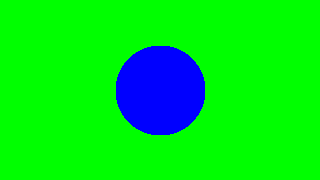
\includegraphics[scale=0.5]{spot}}

Our world consists, not of the Mandelbrot set,
but of the set of points inside a circle of radius one, centered on the origin.
We will build a vewer to look at this marvelous
set, coloring the set blue and everything else 
green.  We will build a program
that will allow us to examine this blue dot
in from any perspective we desire.  


\item[Screen coordinates and world coordinates:]
The first challenge in producing the spot
is the transition between screen coordinates
and world coordinates.  The screen coordinates,
\lstinline{(i, j)} range from 0 to \lstinline{width}
and 0 to \lstinline{height}.

But we want to look at a circle that is centered
on the origin, with unit radius, and we want this
circle centered in our image as in the figure.

In world coordinates, the {\bf center} of the image
is the point $(0,0)$.  The center of the top
is two units above the center, $(0,2)$
and the center of the bottom is a point
two units below the center, $(0,-2)$.  We call the
distance in world coordinates between the center
of the image and the top of the screen the {\bf radius}
of the image.

Clearly, given the row between 0 and \lstinline{height},
we need to lerp this value into the range $0 \pm 2$.
Or, more generally, into the range $center_y \pm radius$.

What about the width?  Any image has an {\bf aspect ratio},
called $R$, which is just the width divided by the height.
Clearly, if the top is $radius$ from the center, in world coordinates, then
the left and right sides are, in world coordinates,
at $center_x \pm R (radius)$.  So, to get from a column
between 0 and $width$ in screen coordinates, we just
have to lerp this number to the interval  $center_x \pm R (radius)$.

This should be enough information to
write a \lstinline{screenToWorld} function
that translates screen coordinates into world coordinates.
\begin{lstlisting}
def screenToWorld(i, j, width, height, center, radius):
    ....
    return (x, y)
\end{lstlisting}


\item[Test data:]  I ran \lstinline{screenToWorld}
with a screen centered at $(0,0)$ and radius of 2, and a width and height
of 640 and 480, and got these numbers for the input 
values of i and j:
\begin{lstlisting}
(0,0) => (-2.6666666666666665, 2.0)
(0,50) => (-2.6666666666666665, 1.5833333333333333)
(0,100) => (-2.6666666666666665, 1.1666666666666665)
(0,150) => (-2.6666666666666665, 0.75)
(50,0) => (-2.25, 2.0)
(50,50) => (-2.25, 1.5833333333333333)
(50,100) => (-2.25, 1.1666666666666665)
(50,150) => (-2.25, 0.75)
(100,0) => (-1.8333333333333333, 2.0)
(100,50) => (-1.8333333333333333, 1.5833333333333333)
(100,100) => (-1.8333333333333333, 1.1666666666666665)
(100,150) => (-1.8333333333333333, 0.75)
(150,0) => (-1.4166666666666665, 2.0)
(150,50) => (-1.4166666666666665, 1.5833333333333333)
(150,100) => (-1.4166666666666665, 1.1666666666666665)
(150,150) => (-1.4166666666666665, 0.75)
\end{lstlisting}
You should be able to get something similar.
You should also be able to compute test values by hand
to check the correctness of your function.

\item[Colorize:] Once you get the world coordinates from
the screen coordinates, finding the color is simple!
For each pixel on the screen at \lstinline{(i, j)}, find the
world coordinates $(x,y)$ for those screen coordinates.
Find the distance from the center, from $(0,0)$ in world coordinates.
This is simply $\sqrt{x^2 + y^2}$.
If this distance is less than 1, it's blue: (0, 0, 255).  
Otherwise,
it's green: (0, 255, 0).

Now we can finally write an image generating program.

\item[Spot with any size screen:]  
Write a program \lstinline{spot.py}
that will display a blue dot in a green field, as above.
You should start with the framework I've given you in
\lstinline{pygamecolors.py} found in the lab's folder.

You should be able to change the height and width
of the image by editing the code.
No matter what the initial height and width are (try it
with several). The spot should be centered horizontally
and vertically, and occupy half the distance from top to
bottom.  It might look like one of these:


\includegraphics[scale=0.5]{spot02}\hfill

\includegraphics[scale=0.25]{spot03}\hfill ~

Do this before going on!

\item[Resizable screen:]  Now rewrite the program
\lstinline{spot.py} to handle resizing the window by dragging a corner.
Your image should
be regenerated at the appropriate size.

To handle resizing a pygame window, you first
have to initialize the screen as follows:
\begin{lstlisting}
screen = pygame.display.set_mode((width,height), pygame.RESIZABLE)
\end{lstlisting}
You also have to handle
the \lstinline{VIDEORESIZE} event, something like this:
\begin{lstlisting}
        elif event.type == VIDEORESIZE:
            width,height = event.dict['size']
            restart(width, height)
\end{lstlisting}
Restarting should reinitialize the screen to the right size,
the background surface we're drawing to, and the pixelsize.
Everything you do when you initialize 
the main loop the first time.  Just do it again.
If you wrote the program by isolating the intitialization
from the main loop, this procedure is probably already
written!

When {\tt spot.py} is run now,
we see our blue spot right where it should be
no matter how we resize the window.

Do this before going on!

\item[Mouse handling:]  Mouse events are handled just
like keyboard events.  I have provided a simple
program, \lstinline{testmouse.py}, that shows how to
get mouse events.

The mouse event handling should be in the same procedure
that handles keyboard events, since all events are put
in the same queue.

\item[Recentering and zooming:]
Suppose we want to change the center of the image
with the mouse?  When we click on a location on the screen,
that should be the new center of view in the world, and furthermore
we should
zoom in on that spot.
For instance, if we left click on the upper right side of the
spot, the screen should redraw with that spot 
(in world coordinates)
as the new center of the screen, and with the image doubled
in size. 

Any mouse click should change the center (in world coordinates)
of the image.  Remember that when you get the mouse event,
it gives you the position of the mouse in {\bf screen} 
coordinates.  You have to change these to world
coordinates before resetting the value of \lstinline{center}.

Clicking the left button should double the size of the
image and clicking the right button should halve the size
of the image.  You can do this wil simple changes to the
\lstinline{radius} of the image.  If you change the
image world coordinates for the vertical range
from $(enter_y \pm 2)$ to $(center_y \pm 4)$ does that make the
things in the image look bigger or smaller?

Clicking the mouse will thus also restart the
program, just like changing window size did.
You should handle mouse events whenever you
handle keyboard or resize events, so just add
the right cases to the event handler.

For example, starting with the figure on the left,
left clicking above and to the right of the spot 
produces the figure on the right:

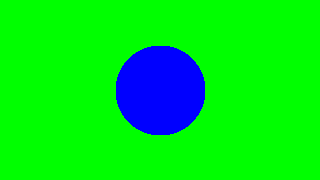
\includegraphics[scale=0.5]{spot}
\hfill

\includegraphics[scale=0.5]{spot04}

We have zoomed in $2\times$ (the spot is twice as big)
and our viewpoint is now above and to the right
of the spot.

Finish this before going on! 
 \lstinline{spot.py}
will be the basis for our Mandelbrot explorer,
which will be {\bf much} more interesting than
a blue spot!



\item[Mandelbrot:]
The Mandelbrot set
pictures are made iterating the  Mandelbrot
function, described in the Wikipedia article.  
If the absolute value goes above 2,
then the series will diverge.  The algorithm simply counts
the number of steps until it goes above 2,
and colorizes according to the number of steps.  
If we go for 250
iterations and it doesn't go above 2, we color it
black.

Starting with \lstinline{spot.py}, copy it to 
\lstinline{mandelbrot.py} and make the following
changes.

There is a pseudocode implementation of the
algorithm in the Wikipedia article.  Implement
this in Python with a function
\begin{lstlisting}
def mandelbrot(x0, y0):
\end{lstlisting}
that returns the number of iterations.

\lstinline{max_iterations} will be a global
variable.  We'll need it elsewhere.   A value of
250 is reasonable for moderate zooming, and reasonably
quick, 
but you can try larger values. 

The colors I used in my Figures I got from 
\href{https://stackoverflow.com/questions/16500656/which-color-gradient-is-used-to-color-mandelbrot-in-wikipedia}{here}.
They are:
\begin{lstlisting}
    colors = [(66,  30,  15),
              (25,   7,  26),
              (9,   1,  47),
              (4,   4,  73),
              (0,   7, 100),
              (12,  44, 138),
              (24,  82, 177),
              (57, 125, 209),
              (134, 181, 229),
              (211, 236, 248),
              (241, 233, 191),
              (248, 201,  95),
              (255, 170,   0),
              (204, 128,   0),
              (153,  87,   0),
              (106,  52,   3)]
\end{lstlisting}
If the number of iterations is \lstinline{n},
we simply take the color at the $n$th
position in \lstinline{colors} list, modulo the length of
the list.
Unless, of course, \lstinline{n == max_iterations},
in which case we color it black.

\item[Adjusting {\tt max\_iterations} (optional):]
If you plan on zooming deeply into the Mandelbrot
set you might want to adjust the \lstinline{max_iterations}.
The finer the detail you need, the larger this should
be.  In my version, whenever I zoomed in (by
changing \lstinline{radius} or out I increased
or decreased the \lstinline{max_iterations} by
a percentage.  There doesn't seem to be any 
good guidance on the ``right'' amount to adjust
this, so, maybe 20\%?

Alternatively, you could use the plus and minus keys
to adjust the \lstinline{max_iterations}, or the
mouse scroll wheel, {\em etc.}

\item[Black is slow!]  The black areas inside
the Mandelbrot set are the ones where the algorithm
had to go to the maximum number of iterations.
These are clearly going to be the slowest points.
If you select regions without so much black,
they'll render faster.

\item[Image names:] When the user presses the S
key a copy of the image is saved.  It is really nice
to know the coordinates and radius of the image,
so you can find it again!  Change the file name
to include the $x$, $y$, and $radius$ used to generate
the image.  

Look at the documentation for \lstinline{format}
in Python.  A fixed format with three digits is
\begin{lstlisting}
'{:.3f}'.format(x)
\end{lstlisting}
This is what I used for my images.

This will also make it nice to browse and save images,
as each image will have a unique name you don't have
to worry about overwriting images when you save new ones.

\item[A new gradient:] Develop your own
color gradient and create at least two nice images
of some interesting places in the Mandelbrot set.
Include these images in your zipped \lstinline{lab09}
folder.

Here is an image I made with a different gradient function:

\showfig{mandX-1.154Y0.352R0.125.png}

\end{description}
\newpage

\centerline{\Large \bf Gallery}

\showfig{mandX-0.688Y0.382R0.00390625.png}


\showfig{mandX-0.009Y0.669R0.03125.png}


\showfig{mandX-1.624Y0.002R0.125.png}


\showfig{mandX0.456Y0.111R0.0625.png}




\end{document}
